% -*- root: ../EstadisticaII.tex -*-

\chapter{Regresión}
El objetivo de la regresión es predecir una/s variable/s en función de la/s otra/s.


\section{Regresión lineal}

Observamos dos variables, X e Y , el objetivo es analizar la relaci´on existente entre ambas, de forma que podamos predecir o aproximar el valor de la variable Y a partir del valor de la variable X.

\begin{itemize}
\item La variable Y se llama variable respuesta.
\item La variable X se llama variable regresora o explicativa.
\end{itemize}

Por ejemplo:
\begin{center}
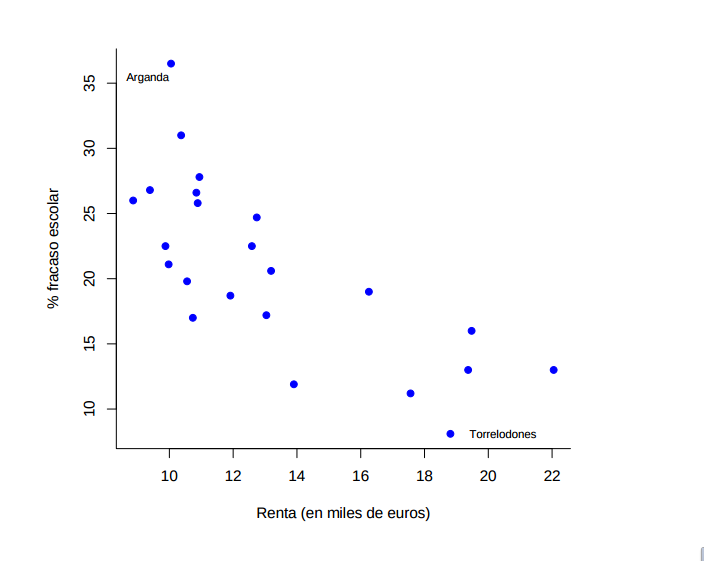
\includegraphics[scale=0.5]{img/RentaVsFracaso.png}
\end{center}

Queremos predecir el fracaso escolar en función de la renta. La variable respuesta es el fracaso escolar, mientras que la variable regresora es la renta. 

\subsection{Regresión lineal simple}

Frecuentemente existe una relación lineal entre las variables. En el caso del fracaso escolar,queremos construir una recta $Y_i = β_0 X_i + β_1\; i=1,...,n$ que minimice el error.

El problema es estimar los parámetros $β_0,β_1$. Una manera de hacer esto es:

\subsubsection{Recta de mínimos cuadrados}

\begin{defn}[Recta de mínimos cuadrados]
Estimando $β_i$ por $\hat{β_i}$ obtenemos: \[\hat{Y_i} = \hat{β}_0 + \hat{β}_1 x_i\]

La reca viene dada por los valores $\hat{β_0}, \hat{β_1}$ para los que se minimiza el error cuadrático, es decir:
\[\sum_{i=1}^n \left(Y_i - \hat{Y_i}\right)^2 =  \sum_{i=1}^n \left[ Y_i - (\hat{β_0} + \hat{β_1}x_i) \right]^2\]
\end{defn}

\begin{example}
\begin{center}
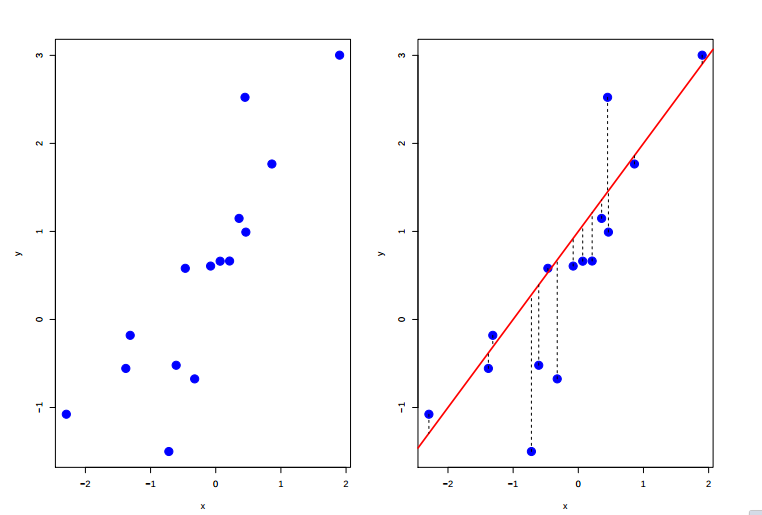
\includegraphics[scale=0.6]{img/ejemploRectaRegresionLineal.png}
\end{center}
\end{example}

\paragraph{Cómo calcular la pendiente} de la recta de mínimos cuadrados.


Vamos a ver unas pocas maneras de calcular la recta de mínimos cuadrados.

\begin{itemize}

	\item El sistema habitual:

	\[ \hat{β_1} = \frac{\sum_{i=1}^n(x_i - \bar{x})(Y_i - \bar{Y})}{\sum_{i=1}^n (x_i - \bar{x})^2} = \frac{S_{xy}}{S_{xx}} \]
	Donde 
		\[S_{xy} = \sum_{i=1}^n(x_i - \bar{x})(Y_i - \bar{Y}) \] 
		\label{Ssubxx}
		\[S_{xx} = \sum_{i=1}^n (x_i - \bar{x})^2\]
	\subitem \[β_0 = \bar{Y} - β_1\bar{x}\]

	\textbf{Entonces:}
	\[\text{recta} \equiv y - \bar{y} = \frac{S_{xy}}{S_{xx}}(x - \bar{x} ) \]

	\item Mínimos cuadrados como promedio de pendientes:
	\label{rmc::promediopendientes}
	\[
	\hat{β_1} = \frac{S_{xy}}{S_{xx}} = \sum_{i=1}^n \frac{(x_i - \bar{x})^2}{S_{xx}} \left( \frac{(Y_i - \bar{Y})}{x_i - \bar{x}} \right) = \sum_{i=1}^n ω_i \left( \frac{(Y_i - \bar{Y})}{x_i - \bar{x}} \right)
	\]

	Vemos que hemos ponderado la pendiente de cada recta que une cada punto con la media. Este peso es mayor cuanto mayor es la distancia \textbf{horizontal}. 

	\item Mínimos cuadrados como promedio de respuestas:

	\[
	\hat{β_1} = \frac{\sum_{i=1}^n  (x_i - \bar{x}) (Y_i - \bar{Y})}{S_{xx}} = \sum α_i Y_i
	\]
	Es interesante ver unas propiedades de estos $α_i$
	\begin{prop}


		\begin{itemize}
			\item[] $\sum α_i = 0$
			\item[] $\sum α_ix_i = 1$
			\item[] $\sum α_i^2 = \frac{1}{S_{xx}}$
		\end{itemize}

	\end{prop}
	\begin{proof}
	\textcolor{red}{Por hacer}
	\end{proof}

\end{itemize}


\begin{defn}[Residuo]
En una recta de mínimos cuadrados: Sea $y_i = β_1x_i - β_0$ y sea $\hat{y}_i = \hat{β}_1x_i - \hat{β}_0$, llamamos residuo a $$e_i = y_i - \hat{y}_i$$

Los residuos cumplen:

\[
\sum_{i=1}^n e_i = 0
\]

Esto es intuitivo, ya que los errores se compensan y además es una buena propiedad.
\end{defn}



\begin{prop}
Sean $\{e_i\}$ una variable aleatoria que cumple \footnote{Se ha utilizado la $e$ porque es útil en cuanto a los residuos de la recta de mínimos cuadrados}:
\[\sum e_i = 0\]

Entonces:
\[\sum e_i x_i = 0 \implies \cov(e,x) = 0\]
\end{prop}

\begin{proof}
\[\sum (e_i - \vec{µ}) x_i = \sum (e_i - \vec{µ}) (x_i - \vx) \]
Por otro lado:

\[
\sum e_ix_i = \sum e_ix_i - \vx \sum e_i = \sum e_i(x_i - \vx)
\]
\end{proof}


\begin{example}
\[
\sum (x_i - \vx)(y_i -\vy) = \sum (x_i - \vx)y_i - \sum \vy\sum(x_i - \vx) \overset{(1)}{=} \sum(x_i - \vx y_i)
\]
\[
(1) \to \sum(x_i - \vx) = 0
\]
\end{example}

Esto tiene la siguiente explicación ``intuitiva'': La recta de mínimos cuadrados contiene toda la información lineal que $X$ puede dar sobre $Y$ (debido a que la covarianza entre los residuos y $X$ es 0).


\subsubsection{Fallos de la recta de mínimos cuadrados}

Vamos a ver un par de ejemplos ilustrativos:

\begin{example}[Sobre los datos atípicos]

Esta es una recta de mínimos cuadrados calculada para una nube de puntos a la que se ha añadido un punto atípico. Se ve una cierta tendencia de que la pendiente debería ser positiva, pero el dato atípico provoca un cambio brusco.
\begin{center}
%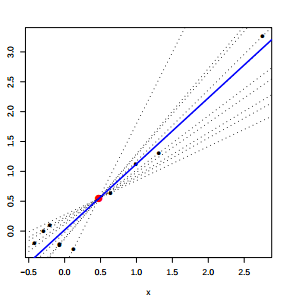
\includegraphics[scale=0.9]{img/rmc_atipico1.png}
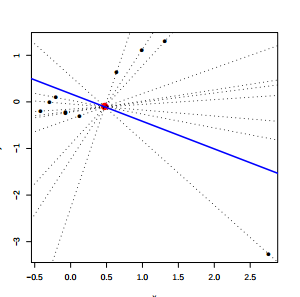
\includegraphics[scale=0.9]{img/rmc_atipico2.png}
\end{center}

\end{example}

\begin{example}[Sobre la distancia horizontal]

¿Y da igual lo atípico que sea un dato? La respuesta es que no. Si el dato es muy atípico en la variable respuesta ($Y$), pero es muy \textit{típico} en la variable regresora, la recta no se devía tanto. Vamos a verlo y después explicamos la razón.

Esta es la recta, en la que hemos ignorado los 3 datos que parecen ``atípicos''.
\begin{center}
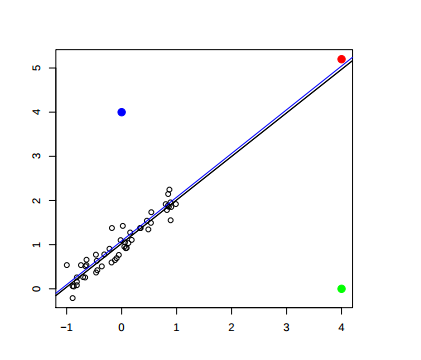
\includegraphics[scale=0.9]{img/sobredistanciahorizontal1.png}
\end{center}

Ahora calculamos las rectas teniendo en cuenta sólo uno de los puntos.

\begin{center}
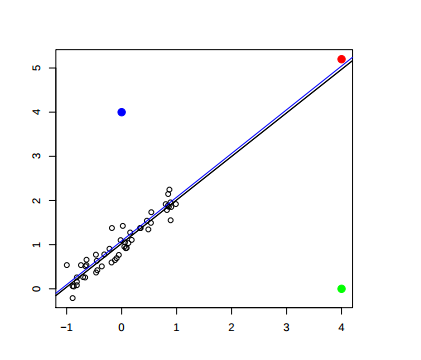
\includegraphics[scale=0.4]{img/sobredistanciahorizontal1.png}
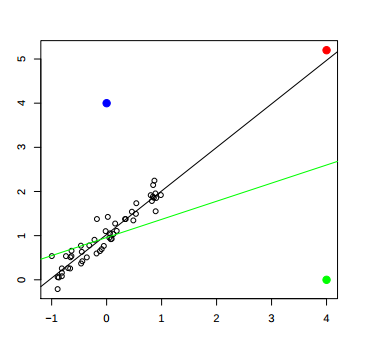
\includegraphics[scale=0.4]{img/sobredistanciahorizontal2.png}
\end{center}

Vemos que la recta azul no se desvía apenas de la original, mientras que la recta verde si se desvía un montón. ¿Esto a qué se debe? A que importa más la distancia horizontal de la media que la distancia vertical. Si vamos a la expresión de la recta de mínimos cuadrados como promedio de las pendientes \label{rmc::promediopendientes} vemos que hay un término $\frac{(x_i - \gor{x})}{S_{xx}}$ que hemos tomado como pesos para ponderar y en este caso, la distancia horizontal $(x_i - \gor{x})$ está multiplicando en el numerador.



\end{example}





\subsubsection{Introduciendo ``aleatoreidad'' para poder hacer IC}

Sea $\{ε_i\}$ siendo $ε_i \sim N(0,σ^2)$. Lo habitual es no saber cómo han sido generados los datos y es probable que no vayamos a conocer con exactitud absoluta la recta de mínimos cuadrados. Es por ello que suponemos el siguiente modelo para la variable respuesta:

\[
Y_i = β_1 x_i + β_0 + ε_i
\]


Tenemos que $\bar{y}_i \sim N$, ya que es una combinación lineal de variables normales \textbf{independientes} (como vimos en el Tema 1). 


\begin{example}
Sea $σ=1, β_0 = 0 y β_1 = 1$.

Entonces el modelo es:

\[
Y_i = x_i + ε_i
\]

Fijamos $n=10$ y generamos las respuestas para $x_i = i$. Además, repetimos el experimento 6 veces y calculamos las rectas de mínimos cuadrados, obteniendo:

\begin{center}
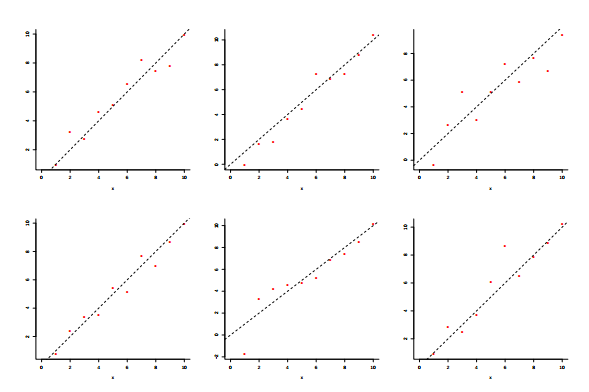
\includegraphics[scale=0.6]{img/6ejemplosRegresion.png}
\end{center}

Vemos que obviamente las rectas no son las mismas. Esto se debe al $ε_i$ introducido. ¿Cuáles son los valores que toman $β_1$ y $β_0$? Habiendo repetido el experimento 1000 veces, obtenemos los siguientes histogramas:

\begin{center}
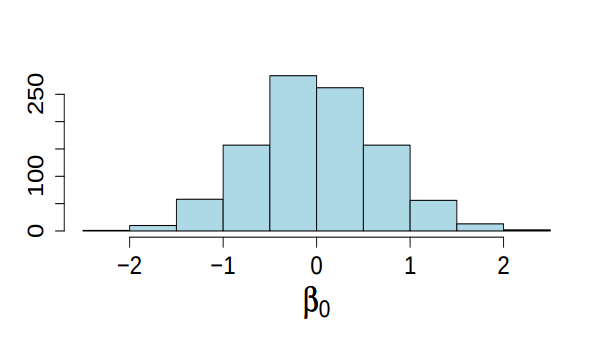
\includegraphics[scale=0.3]{img/1000vecesb0.png}
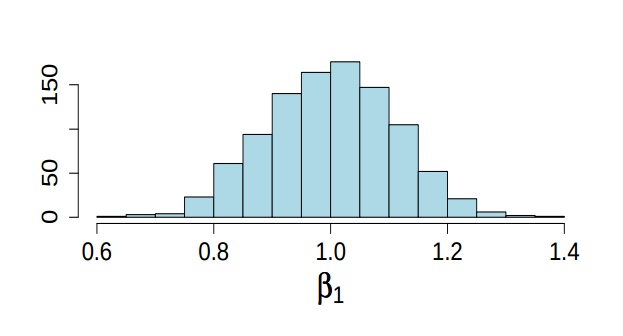
\includegraphics[scale=0.3]{img/1000vecesb1.png}
\end{center}

Vemos que no siempre es el mismo valor. Sabemos (por cómo hemos construido los datos) que $β_0 = 0$ y $β_1 = 1$, pero nuestra manera de calcularos (debido a $ε_i$) no siempre nos da el valor concreto. 


\end{example}

El ejemplo anterior nos muestra que en realidad, estamos estimando $β_i$, aunque no nos guste y ahora tenemos que planternos ¿cómo de buenos son nuestros estimadores? Tal vez son una mierda, o tal vez son insesgados. 

Para ello, vemos que al haber añadido un error $\epsilon_i \sim N(0,σ^2)$, tenemos:

\[
Y_i = β_0 + β_1x + ε_i \implies Y_i \equiv N(β_0 + β_1X_i, σ^2)
\] 


\subsubsection{Estimando $β_1$}

\begin{prop}
Nuestro estimador ``pendiente de la recta de mínimos cuadrados:'' $\hat{β_1}$  cumple

\[
\hat{β_1} \equiv N\left(β_1,\frac{σ^2}{S_{xx}} \right)
\]

\end{prop}

\begin{proof}
Él en clase lo ha hecho al revés. Muchos cálculos para llegar a la conclusión, pero aquí molamos más. En algún momento \textcolor{red}{revisará} alguien los apuntes y completará.

\begin{itemize}
	\item $\esp{\hat{β_1}} = β_1$
	\item $\var{\hat{β_1}} = ... = \displaystyle\frac{σ^2}{S_{xx}}$
\end{itemize}
\end{proof}

\subsubsection{Estimando $β_0$}

\begin{prop}
Nuestro estimador ``término independiente de la recta de mínimos cuadrados:'' $\hat{β_0}$  cumple

\[
\hat{β_0} = N\left(β_0 , σ^2 \left( \frac{1}{n} + \frac{\gor{x}^2}{S_{xx}}\right)  \right)
\]
\end{prop}

\begin{proof}
\begin{itemize}
	\item $\esp{\hat{β_0}} = β_0$
	\item 
	$\var{\hat{β_0}} = \var{\gor{Y}} + \var{\hat{β_1}\gor{X}} - 2 \cov\left(\gor{Y},\hat{β_1}\gor{X}\right)$

 	\subitem Calculamos: $\cov\left(\gor{Y},\hat{β_1}\gor{X}\right)$ utilizando cosas del tema 1

 	\[
		\cov\left(\gor{Y},\hat{β_1}\gor{X}\right) = \cov\left(\frac{1'_n \gor{Y}}{n},α\gor{Y}\right) = \frac{1}{n}1'_nσ^2
 	\]
 	debido a que $α = 0$.

 	Ademas de ser incorrelados, son \textbf{independientes}. ¿Porqué? Porque conjutamente son normales, es decir \[
 		\begin{pmatrix} \gor{Y} \\ \hat{β_1} \end{pmatrix} \equiv A\gor{Y} \equiv N_2
 	\]
\end{itemize}

\end{proof}


\textbf{Conclusiones:}
\begin{align*}
\gor{Y} &\text{ es indepediente de } \hat{β_1}\\
\hat{β_1} &\equiv \left(β_1,\frac{σ^2}{S_{xx}}\right)\\
\hat{β_0} &\equiv \left(β_0,σ^2 \left( \frac{1}{n} + \frac{\vec{x}^2}{S_{xx}}\right)\right)
\end{align*}

¿Son estas las variables $\hat{β_1} $ y $\hat{β_2}$ normales una normal conjunta? No, \textbf{no son una normal conjunta} ya que no son independientes. Intuitivamente es fácil de ver. En una recta, si aumentamos la pendiente (y estamos en el primer cuadrante) entonces el término independiente disminuye. Esta dependencia tiene que aparecer. Vamos a estudiar la covarianza entre los estimadores:

\[
\cov\left(β_1,β_2\right) = \cov\left(\gor{Y} - \hat{β_1}\gor{x}, \hat{β_0}\right) = ... = -\gor{x}\frac{σ^2}{S_{xx}}
\]



\subsubsection{IC y Contrastes para $β_1$}

Recordamos que \[ \hat{β}_1 \equiv N\left(β_1,\frac{σ^2}{S_{xx}}\right)\]

Podemos normalizar y buscar una catidad pivotal (como hacíamos en estadística I)

\[
\frac{\hat{β_1} - β_1}{\frac{σ}{S_{xx}}} \equiv N\left(0,1\right)
\]

Pero aquí nos encontramos con que necesitamos $σ$, la varianza de los errores. Esta varianza a menudo no es conocida (porque no sabemos con exactitud cuál es la recta verdadera) y tenemos que estimarla. 

Para estimarla, parece razonable usar \[ \hat{σ} = S_R =\frac{\sum_{i=1}^n e_i^2}{n-2}\] 

\begin{expla}
Recordamos que para que estimar la varinza, utilizamos (por el lema de fisher) $n-1$ de denominador para que el estimador sea insesgado. Esto sale de que en la demostración, hay una matriz de rango $n-1$ ya que existe una restricción.

Siguiendo este razonamiento, en este caso tenemos 2 restricciones\footnote{$\sum e_i = 0$ y $\sum e_ix_i = 0$}, por lo que si lo demostráramos rigurosamente, aparecería una matriz de rango $n-2$ y por eso es el denomiador. De esta manera, conseguimos un estimador insesgado.

\end{expla}

Además, $S_R$ se denomina \concept{varianza residual}

\begin{prop}
Una pequeña generalización del lema de Fisher:
\[
\frac{(n-2)S_{R}^2}{σ^2} \equiv \chi_{n-2}^2
\]

Además, es independiente de $\hat{β_1}$

\end{prop}



\begin{proof}
Esta proposición es un caso particular de un teorema que veremos más adelante.
\end{proof}


Ahora que ya tenemos estimada la varianza, podemos calcular:


\[
\frac{\hat{β_1}-β_1}{\frac{S_R}{\sqrt{S_{xx}}}} = \frac{\hat{β_1}-β_1}{\displaystyle\frac{\frac{σ}{\sqrt{S_{xx}}}}{\frac{S_R}{σ}}}
\]

En el numerador tenemos una $N(0,1)$ y en denominador una $\chi^2$ dividida por sus grados de libertad. Esto es por definición de $\mathcal{T}$ \footnote{T de Student} es una $\mathcal{T}$ (T-Student) con $n-2$ grados de libertad.

\begin{prop}
Ahora que conocemos la distribución, podemos calcular el intervalo de confianza  para la pendiente de la recta.

\textcolor{red}{No entiendo nada de esto.}
\[
IC_{1-α}(β_1) \equiv \left[ \hat{β_1} \pm \mathcal{T}_{n-2,\frac{α}{2}}\frac{S_R}{\sqrt{S_{xx}}}\right] \equiv \left[ \gor{Y} \pm \mathcal{T}_{n-1,\frac{α}{2}}\frac{S_R}{\sqrt{n}} \right]
\]
\end{prop}

\subsubsection{Contraste en R}


\begin{lstlisting}
> # Ajusta el modelo
> regresion = lm(Fracaso~Renta)
> summary(regresion)

> lm(formula = Fracaso ~ Renta)
Residuals:	Min	1Q	Median	3Q	Max
		-7.8717 -3.7421	0.5878	3.0368	11.5423
---
Coefficients:	Estimate Std.	Error 	t-value	Pr(>|t|)
(Intercept)	38.4944		3.6445	10.562	7.37e-10 ***
Renta 		-1.3467		0.2659	-5.065	5.14e-05 ***
---
Signif. codes: [...]
Residual standard error: 4.757 on 21 degrees of freedom
Multiple R-Squared: 0.5499,
Adjusted R-squared: 0.528
\end{lstlisting}


Aquí, la fila de intercept es el término independiente y renta es la pendiente. Además, los p-valores son para el contraste $\hat{β_i} = 0$, dentro de la hipótesis $β_i \geq 0$. \footnote{Si queremos contrastar si es positivo, nos vamos al caso límite que lo separa y contrastamos eso}.

En este caso, el p-valor para $\hat{β_1} = 7.37e-10$, con lo que no podemos rechazar la hipótesis.


\subsubsection{Predicciones}

Sea $(x_1,y_1),...,(x_n,y_n) \to y_i = β_0 + β_1x_i + ε_i$.

Dado una nueva observación $x_0$, tenemos 2 problemas para predecir:

\begin{itemize}
	\item Inferencia sobre $m_0 \equiv \esp{y_0 | x_0} = β_0 + β_1x_0$

	En este caso, $$\hat{m_0} = \hat{β_0} + \hat{β_1}x_0$$

	¿Cómo es este estimador?

	\[\esp{\hat{m_0}} = β_0 + β_1x_0 = m_0\]
	\[\var{\hat{m_0}} = ... = σ^2\left[\frac{1}{n} + \frac{(x_0-\bar{x})^2}{S_{xx}} \right] \]

	\subitem Intuitivamente, lo que significa el segundo sumando de la varianza es que ``cuanto más cerca esté $x_0$ de la media, mejor será la estimación''.

	\textbf{Conclusión:}

	\[
		\hat{m_0} \sim N\left( m_0, σ^2\left[\frac{1}{n} + \frac{(x_0-\bar{x})^2}{S_{xx}} \right]\right)
	\]



	\subitem \textbf{Intervalo de confianza} para $m_0$ utilizando la fórmula de intervalos de confianza:

	\[
IC_{1-α}(m_0) \equiv \left[ \hat{m_0} \pm \mathcal{T}_{n-2,\frac{α}{2}}S_R\sqrt{\frac{1}{n} + \frac{(x - \gor{x})^2}{S_{xx}}}\right] 
\]

	\item Predecir $Y_0$ usamos de nuevo:

	\[
\hat{Y_0} = \hat{β_0} + \hat{β_1}x \to Y_0 - Y \equiv N\left( 0, σ^2\left( 1 + \frac{1}{n}+  \frac{(x-\gor{x})^2}{S_{xx}}\right) \right)
	\]

	Donde la varianza ha sido calculada:

	\[
	\var{Y_0 - \hat{Y_0}} = \underbrace{\var{Y_0}}_{σ^2} - \var{\hat{Y_0}} + \underbrace{2 \cov{Y_0,\hat{Y_0}}}_{ = 0 \text{ (indep.) }} = σ^2 + σ^2\left( \frac{1}{n}+  \frac{(x-\gor{x})^2}{S_{xx}} \right)
	\]


	Este es un problema más complicado, ya que tenemos que tener en cuenta el término de error $ε_i$ y es por esto que aparece el 1 en la varianza. Tenemos que tener en cuenta la incertidumbre.

	Estandarizando y cambiando $σ$ por $S$, tenemos:

	\[
	\frac{Y_0 - \hat{Y_0}}{S_r \sqrt{1 + \frac{1}{n} + \frac{(x-\gor{x})^2}{S_{xx}}}} \equiv \mathcal{T}_{n-2} 
	\]

	Ya que tenemos una normal estandarizada dividida por su .... que por definición, es una $\mathcal{T}$ de student.

	Ahora, vamos a construir el \concept{intervalo de predicción} (cambia ligeramente la interpretación)

	\[
1 - α = P\left\{ -\mathcal{T}_{n-2;\frac{α}{2}} < \frac{Y_0 - \hat{Y_0}}{...} < \mathcal{T}_{n-2;\frac{α}{2}}    \right\} = P \left\{ Y_0 \in \left[ \hat{Y_0} \pm \mathcal{T}_{n-2;\frac{α}{2}} S_R \sqrt{1+\frac{1}{n}+...} \right]  \right\}
	\]
\end{itemize}

Ahora vamos a hacer unos ejemplos numéricos.



\subsection{Regresión lineal múltiple}


\subsection{Estimadores de mínimos cuadrados}
\subsection{Inferencia sobre los parámetros del modelo}
\subsection{Análisis de la varianza}
\subsection{Contrastes de hṕótesis lineales}
\subsection{Modelo unifactorial}